% Preamble
% Compile with XeLateX

\documentclass[11 pt,oneside,a4paper,titlepage]{article}
\usepackage{preamble}
\graphicspath{{PIC/}}
%%%%%%%%%%%%%%%%%%%%%%%%%%%%%%%%%%%%%%%%%%%%%%%%%%%%%%%%%%%%%%%%%%%%%%%%%%%%%%%%%%%%%%
\begin{document}

\sidebar{sideBarColor!25}
\simpleheader{titleBackColor}{}{Serli Kopar}{ Second year FOKUS Life Sciences M.Sc.}{white}

% Start Minipages
\vspace*{3.49cm}% start 8 cm from the top of the page}
    \adjustbox{valign=t}{\begin{minipage}{7.3cm} % large 7.4 cm from the top
    \vspace*{1.2cm} % text starts 1cm under the top of the mPnipage
            
        % Picture
        \begin{center}
        \begin{tikzpicture}
            \node[
            circle,
            minimum size=\cvPictureWidth,
            path picture={
            \node at (path picture bounding box.center){
             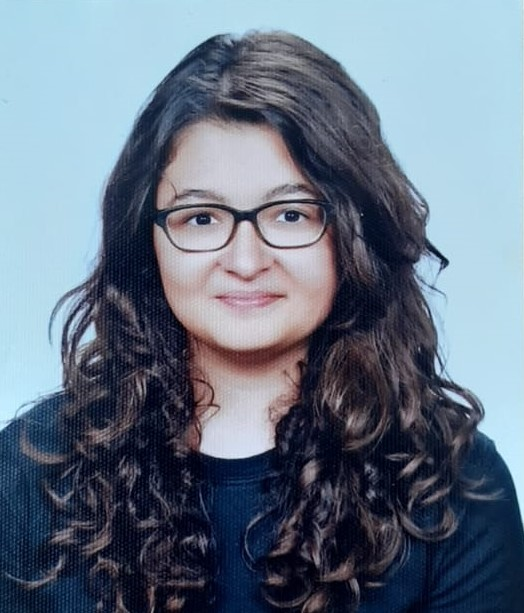
\includegraphics[width=\cvPictureWidth]{Vesika3_1.jpg}
             };
             }]
            {};
        \end{tikzpicture}
        \end{center}

        %%%%%%%%%%%%%%%%%%%%%%%%%%%%%%%%%%%%%%%%%%%%%%%%%%%%
        % Profile section
        %\ruleline{\textbf{About me}}
        %\lipsum[150] %
        
        %%%%%%%%%%%%%%%%%%%%%%%%%%%%%%%%%%%%%%%%%%%%%%%%%%%
        % Contact Section
        \section*{{\faThumbTack} PERSONAL DATA}
        %\ruleline{\textbf{Personal Data}}
        \begin{tikzpicture}[every node/.style={inner sep=0pt, outer sep=0pt}]
        \matrix [
        column 1/.style={anchor=center,contactIcon},
        column 2/.style={anchor=west,align=left,contactIcon},
        column sep=5pt,
        row sep=5pt] (contact) {
        \node{\faFemale};
         & \node{Born on 05/05/2000 | Age 24};\\
        \node{\faEnvelope}; 
         & \node{\href{mailto:serli.kopar@stud-mail.uni-wuerzburg.de}{serli.kopar@stud-mail.uni-wuerzburg.de}};\\
         \node{\faEnvelopeO}; 
         & \node{\href{mailto:serlikopar@hotmail.com}{serlikopar@hotmail.com}};\\
        \node{\faPhone}; 
         & \node{+49 176 322 900 90};\\ 
        \node{\faMapMarker}; 
        & \node{Am Galgenberg 52 | 97074, Würzburg};\\
        \node{\faLinkedinSquare}; 
        & \node{\href{https://www.linkedin.com/in/serli-kopar-05599b232/?locale=de_DE}{serli-kopar}};\\
        %\node{\aiResearchGateSquare}; 
        %& \node{\href{https://www.researchgate.net/scientific-contributions/Serli-Kopar-2244245642}{Research Gate: Serli Kopar}};\\
        \node{\aiOrcid}; 
        & \node{\href{https://orcid.org/0000-0002-1409-2896}{ORCID: 0000-0002-1409-2896}};\\
       % \node{\faCar};
       % & \node{Car Available, Driving License B};\\
         };
        \end{tikzpicture} 
        \vspace{0.4cm}
        %%%%%%%%%%%%%%%%%%%%%%%%%%%%%%%%%%%%%%%%%%%%%%%%%%%
        \section*{{\faLanguage} LANGUAGES}
        %\ruleline{\textbf{Languages}}
        \begin{tikzpicture}[every node/.style={inner sep=0pt, outer sep=0pt}]
        \matrix [
        column 1/.style={anchor=center,contactIcon},
        column 2/.style={anchor=west,align=left,contactIcon},
        column sep=5pt,
        row sep=5pt] (contact) {
        \node{\flag{tur.png}};
        & \node{Turkish - Native Language};\\
        \node{\flag{ger.png}};
        & \node{German - C1 - DSD2: 90/96};\\
        \node{\flag{England.png}};
        & \node{English - C1 - TOEFL: 106/120};\\
        \node{\flag{rus.png}};
        & \node{Russian - B1 - University Certification};\\
        \node{\flag{Spain.png}};
        & \node{Spanish - B1 - University Certification};\\
        };
        \end{tikzpicture} 
        \vspace{0.4cm}
        %%%%%%%%%%%%%%%%%%%%%%%%%%%%%%%%%%%%%%%%%%%%%%%%%%%second
        \section*{{\faHeartbeat} AWARDS HONOURS}
        %\ruleline{\textbf{Academic Honours and Awards}}
        \begin{tikzpicture}[every node/.style={inner sep=0pt, outer sep=0pt}]
        \matrix [
        column 1/.style={anchor=center,contactIcon},
        column 2/.style={anchor=west,align=left,contactIcon},
        column sep=5pt,
        row sep=5pt] (contact) {
        \node{\flag{daad.png}};
        & \node{DAAD Full Scholarship 10/19 -/10/22};\\
        \node{\flag{tüb.png}};
        & \node{National Chemistry Olympiad in Turkey \\
Third place in the district 25/10/18};\\
        \node{\flag{ros.jpg}};
        & \node{Undergrad Rostock Scholarship  07/18};\\
       % \node{\flag{rus.png}};
       % & \node{Russian - B1 - University Certification};\\
       % \node{\flag{Spain.png}};
       % & \node{Spanish - B1 - University Certification};\\
        };
        \end{tikzpicture} 
        \vspace{0.4cm}
        %%%%%%%%%%%%%%%%%%%%%%%%%%%%%%%%%%%%%%%%%%%%%%%%%%%
         \section*{{\faFolderOpen} CERTIFICATES}
        % \ruleline{\textbf{Certificates}}
        \begin{tikzpicture}[every node/.style={inner sep=0pt, outer sep=0pt}]
        \matrix [
        column 1/.style={anchor=center,contactIcon},
        column 2/.style={anchor=west,align=left,contactIcon},
        column sep=5pt,
        row sep=5pt] (contact) {
        \node{\flag{code.png}};
        & \node{\href{https://www.codecademy.com/profiles/method8211391069/certificates/451f96e6ed7270d49283e833c58285fd}R for Programmers};\\
        \node{\flag{code.png}};
        & \node{\href{https://www.codecademy.com/profiles/method8211391069/certificates/5d24b4845808221825fadca1}Visualize and Analyze Data with Python};\\
        \node{\flag{code.png}};
        & \node{\href{https://www.codecademy.com/profiles/method8211391069/certificates/c87ba0541f8be78bc2f4ba1128233f6f}Command Line Linux and Python 3};\\
        \node{\flag{john.png}};
        & \node{\href{https://www.coursera.org/account/accomplishments/certificate/RBHCC32FEQGF}Introduction to Genomic Technologies};\\
        \node{\flag{john.png}};
        & \node{\href{https://www.coursera.org/account/accomplishments/certificate/KWHPHKTTWWPA}Python for Genomic Data Science};\\
        \node{\flag{dtu.png}};
        & \node{\href{https://www.coursera.org/account/accomplishments/certificate/HGWA7XRHY9JV}Whole Genome Sequencing of Bacterial\\
Genomes Tools and Applications};\\
        };
        \end{tikzpicture} 
        
    \end{minipage}} %
    \hfill 
%%%%%%%%%%%%%%%%%%%%%%%%%%%%%%%%%%%%%%%%%%%%%%%%%%%%%%%%%
%%%%% MAIN SECTION %%%%%%%%%%%%%%%%%%%%
    \adjustbox{valign=t}{\begin{minipage}{11.3cm}
        \vspace*{1cm}
        \section*{{\faGraduationCap} EDUCATION}

        \MySection{2022-Ongoing}{wur.png}{Master's Degree}{University of Würzburg}{Würzburg, Germany}{Faculty of Biology}{International FOKUS Life Sciences Fast-track M.Sc.  \\\textbf{Minor in Computer Science - since 04/2023} \\ Selected Lectures: \textit{Single Cell Sequencing, Machine Learning for Natural Language Processing \& Complex Networks, Data Mining, Reinforcement Learning for Decision Making \& Optimal Control}\\\textbf{Overall GPA: 1.0}}
            
        \vspace*{0.22cm}
            
        \MySection{2019-2022}{fau.png}{Bachelor's Degree}{University of Erlangen-Nürnberg}{Erlangen, Germany}{Faculty of Medicine}{Molecular Medicine Selected Lectures: \textit{Microbiology, Immunology and Virology, Neurophysiology and Neuroanatomy, Human Genetics, Biometry and Epidemiology,Pharmacology and Toxicology}}
                
        %%%%%%%%%%%%%%%%%%%%%%%%%%%%%%%%%%%%%%%%%%%%%%%%%%%
        % Work Experience
        \section*{{\faSuitcase} RESEARCH ACTIVITIES}
        \MySection{08/23-Today}{sys.png}{Internship \& Master's Thesis}{Max Planck Research Group for Systems Immunology}{Würzburg}{ML in Single cell RNA-sequencing}{Prof. Dr. rer. nat. Dominic Grün - I am developing algorithms using Graph Neural Networks (GNNs) and Natural Language Processing (NLP) tasks to benchmark single-cell sequencing analysis methods. Enhancing latent space representations to integrate spatial data, focusing on explainable AI and causal inference to understand cell-cell communication and cell-fate decisions.}  
            
        \vspace*{0.22cm}
        \MySection{12/23-08/24}{tum.png}{AI Tutor}{Technical University of Munich}{remote} {Pivotal role in a statewide educational initiative}{
As an AI Tutor at the Technical University of Munich, I fine-tuned a local Mistral 7B model to create a chatbot for physio-chemistry lectures and medical case assistance. I also enhanced educational experiences by enriching course materials, creating quizzes, developing multimedia resources, and organizing workshops and events.
}  
        
        
        \MySection{09/22-05/23}{hiri.png}{Three Internship Rotations}{Helmholtz Institute for RNA-based Infection}{Würzburg}{Nanopore sequencing and CRISPR ML applications}{Prof. Dr. Antoine-Emmanuel Saliba - Bioinformatical Analysis of Single Cell Sequencing Data \\
        Jun.-Prof. Dr. Lars Barquist - Developement of automated machine learning prediction
models to quantify bacterial CRISPRi guide efficiency \\ Jun.-Prof. Dr. Redmond Smyth -Nanopore Sequencing of Vaccinia, Comparative Bioinformatical
Analysis of Flongle vs Minion Cells }  
            
        \vspace*{0.22cm}

        \MySection{10/21-08/28}{klinik_E.png}{Bachelor’s Thesis \\\& Student 
Laboratory Assistant}{Virological Institute of the University Hospital}{Erlangen}{Cancer drugs repurposing}{Prof. Dr. rer. nat. Manfred Marschall- Developement of experimental approaches to exploit
the cytomegalovirus nuclear egress complex as an antiviral
target
}  
            
        \vspace*{0.22cm}

       \MySection{05/21-12/20}{math.png}{Student Research Assistant}{Institute of Mathematics - Chair of Analytics Mixed-
Integer Optimization}{Erlangen}{COVID 19 data mining }{Dr. Bismark Singh- Implementation of mathematical models to investigate
equitable allocation of vaccines for Covid-19 strategies
}
            
      %  \vspace*{0.22cm}

    %    \MySection{02/21-04/21}{karow.png}{Internship}{Karow Lab}{Erlangen}{Concentrating predominantly on organoid growth}{Prof. Dr. rer. nat. Marisa Karow- Study of new molecular targets for navigating and correcting
%defective neurogenesis}
            
         
        %%%%%%%%%%%%%%%%%%%%%%%%%%%%%%%%%%%%%%%%%%%%%%%%%%%
        
     \end{minipage} %  
    
%%%%%%%%%%%%%%%%%%%%%%%%%%%%%%%%%%%%%%%%%%%%%%%%%%%%%%%%%%%%
% Second Page
\newpage

\sidebar{sideBarColor!25}
\newpageheader{titleBackColor}{}{Serli Kopar}{Graduate Student \faLightbulbO \hspace{1.5mm} Research Assistant}{white}

% %%%%%%%%%%%%%%%%%%%%%%%%%%%%%%%%%% SIDEBAR %%%%%%%%%%%%%%%%%%%
\adjustbox{valign=t}{%
\begin{minipage}{7.3cm} 
\vspace*{0.4cm} % text starts 0.4cm under the top the header
        
    %%%%%%%%%%%%%%%%%%%%%%%%%%%%%%%%%%%%%%%%%%%%%%%%%%%%
    % Skill and Strengths 
    \section*{{\faGithub} COMPUTATIONAL SKILLS}
    % \ruleline{\textbf{Information Technology Skills}}
    \vspace*{0.25cm}
    \begin{center}

        \cvtag{PyTorch /& PyG} \cvtag{Large Language Models} \cvtag{Graph Learning} \cvtag{Statistics}  \cvtag{Information Theroy} \cvtag{Analysis of Sequencing Data}  \cvtag{Docker/Anaconda/VCS Proficiency}
        \cvtag{Nanopore \& Single cell sequencing}\cvtag{Python}\cvtag{R}\cvtag{MATLAB}\cvtag{\LaTeX} \cvtag{SQL} 
        %\cvtag{MS Office} 
    \end{center}

    %%%%%%%%%%%%%%%%%%%%%%%%%%%%%%%%%%%%%%%%%%%%%%%%%%%%
    % Professional Skills 
    \section*{{\faFlask} LAB SKILLS}
    %\ruleline{\textbf{Lab Skills}}
    \begin{center}
        \cvtag{Cell Culture S1-S3} \cvtag{PCR}\cvtag{Western Blot}\cvtag{Immuno-histo chemistry}\cvtag{Purification}\cvtag{Animal Experiments}
    \end{center}

    \section*{{\faBook} PUBLICATIONS}
    \small
    \\
    \footnotesize {An antiviral targeting strategy based on the inducible interference with cytomegalovirus nuclear egress complex} Kicuntod, J., Häge S., Lösing J., \textbf{Kopar S.} , Muller Y.A., Marschall Manfred, April 2023,\href{https://doi.org/10.1016/j.antiviral.2023.105557}{DOI: 10.1016/j.antiviral.2023.105557}
    

    \vspace{0.4cm}
    
    \footnotesize \textbf{The Oligomeric Assemblies of Cytomegalovirus Core Nuclear Egress Proteins Are Associated with Host Kinases and Show Sensitivity to Antiviral Kinase Inhibitors}, May 2022,\href{https://doi.org/10.3390/v14051021}{DOI: 10.3390/v14051021}
    \\
    \vspace{0.22cm}

    \section*{{\faBalanceScale} EXTRA-CURRICULARS}
        \begin{tikzpicture}[every node/.style={inner sep=0pt, outer sep=0pt}]
        \matrix [
        column 1/.style={anchor=center,contactIcon},
        column 2/.style={anchor=west,align=left,contactIcon},
        column sep=5pt,
        row sep=5pt] (contact) {
        \node{\flag{pasch.png}};
        & \node{PASCH Alumni Association Elected Speaker \\PASCH Mentoring-Program - since 05/22 };\\
        \node{\flag{eelisa.jpg}};
        & \node{European Engineering Learning Innovation\\
Science Alliance Board Member - since 04/21};\\
        \node{\flag{daad.png}};
        & \node{DAAD Online Event Organisator };\\
        \node{\flag{stbil.png}};
        & \node{Studenten bilden Schüler e.V. - 05/21-08/22 \\
Teaching students with migration background};\\
        \node{\flag{instco.png}};
        & \node{Commission for Internationalization- SS 22};\\
        };
        \end{tikzpicture} 

        
    %%%%%%%%%%%%%%%%%%%%%%%%%%%%%%%%%%%%%%%%%%%%%%%%%%%
    % Other Interests
    \section*{{\faBullhorn} REFERENCES}
    %\ruleline{\textbf{References}}
   % \small
    %\begin{multicols}{2}
        \begin{itemize} 
            \item  Prof. Dr. Dominic Grün, \newline  \href{mailto:dominic.gruen@uni-wuerzburg.de}{dominic.gruen@uni-wuerzburg.de}
             \item  Prof. Dr. Ingo Scholtes, \newline  \href{mailto:ingo.scholtes@uni-wuerzburg.de}{ingo.scholtes@uni-wuerzburg.de}
              \item  Prof. Dr. Manfred Marschall,\newline  \href{mailto:manfred.marschall@fau.de}{manfred.marschall@fau.de}
    \end{itemize}
    %\end{multicols}

     

\end{minipage}
}%
\hfill
%%%%%%%%%%%%%%%%%%%%%%%%%%%%%%%%%%% MAIN %%%%%%%%%%%%%%%%%%%%%%%%%
\adjustbox{valign=t}{%
\begin{minipage}{11.3cm}
    \vspace*{0.4cm}
     \section*{{\faSuitcase} WORK EXPERIENCE}
     
         \MySection{08/24-Today }{CAIDAS_quer_4.png}{Machine Learning Engineer}{Centre for Artificial Intelligence and Data Science}{Würzburg}{Main Goal: Improving the contextual understanding of Large Language Models (LLMs)}{Incorporating Contextual Adapters and Fine-Tuning Techniques for superior context awareness. }  
            
        \vspace*{0.22cm}
        
        \MySection{07/24-Today }{klinik_W.png}{Conversational AI Engineer }{ENT Clinics of University Hospital}{Würzburg}{Main Goal: Eenhancing the efficiency of clinical training}{Developing chatbots to assist clinicians in their practical year (PJ) with case-based decision-making and to help medical students prepare for their exams.}  
            
        \vspace*{0.22cm}
        
        \MySection{10/23-Today }{sys.png}{Research Assistant}{Max Planck Research Group for Systems Immunology}{Würzburg}{Main Method: Mice Genotyping}{Assisting senior researchers with mouse and transduction experiments}  
            
        \vspace*{0.22cm}
         \MySection{10/23-04/24}{wur.png}{Teaching Assistant}{University of Würzburg}{Würzburg}{Main Method: Grading students based on weekly assignments}{Lecture Series "Methods in Life Sciences" for Bio-sciences Master Students}  
            
        \vspace*{0.22cm}
         \MySection{10/22-01/24}{klinik_W.png}{Student Assistant in Diagnostics}{University Hospital Würzburg}{Würzburg}{Main Method: ELISA and PCR}{Testing swap, blood and urin samples of patients for diagnosis and clinical studies}  
            
        \vspace*{0.22cm}
        
        \MySection{04/22-
09/22}{fau.png}{Research Data Analyst}{Institute for Medical Informatics, Biometry and Epidemiology
(IMBE)}{Erlangen}{Main Method: MatLab + RStudio}{Prof. Dr. rer. nat.Olaf Gefeller-Developement of connected models and investigation
of epidemiological risk concepts for clinical studies
}  
            
        \vspace*{0.22cm}

        \MySection{04/22-
09/22}{emil.jpg}{Teaching Assistant}{Emil Fischer Centre}{Erlangen}{Grading students based on weekly assignments}{Lecture Series "Biochemistry 1 and 2" for
Medical Students}  
            
       

     %   \vspace*{0.22cm}

        
    %%%%%%%%%%%%%%%%%%%%%%%%%%%%%%%%%%%%%%%%%%%%%%%%%%%
    % Peer Reviews
   % \section*{{\faBook} PUBLICATIONS}
   % \footnotesize I did academic peer review for the following journals: 
    %\begin{itemize}
   % \footnotesize{An antiviral targeting strategy based on the inducible interference with cytomegalovirus nuclear egress complex}, \href{https://doi.org/10.1016/j.antiviral.2023.105557}
     %\end{itemize}

    \section*{{\faMicrophone}  TALKS \& WORKSHOPS GIVEN BY ME}

    \footnotesize \textbf{Level Up Your Machine Learning: Hands-on Exploration of Linear Models to Deep Learning}{ @Max Planck Systems Immunology lab retreat, June 21 2024. In this workshop, I showed participants the power of machine learning through a hands-on exploration. We started by building a foundation in linear models, then I used Multi-Layer Perceptrons (MLPs) to introduce the concept of neural networks. Finally, we delved into the exciting world of Graph Neural Networks (GNNs) and explored various Deep Learning techniques.}

    \vspace{0.5 cm}
   
    \footnotesize \textbf{Fine-Tuning the Future: AI-Powered Chatbots Revolutionize Physico-Chemical Education in Lectures } {@6. Symposium of WueDive and QUADIS},May 24 2024. As an AI tutor, I developed a chatbot for physico-chemical lectures using the Mistral7B base model for fine-tuning, leveraging lecture notes as training data which were carefully preprocessed. This model was successfully presented in this talk and is currently implemented in lectures, enhancing student learning by overcoming communication barriers and providing flexible study times.}
    
    \vspace{0.5 cm}
    
    \footnotesize \textbf{Unleashing the Power of LLMs: A Hands-on Workshop on Prompting Techniques for Educators Across Disciplines}{ @Day of Good Teaching of the Bavarian State Ministry of Science and Art, April 10 2024. In this interactive workshop, I equipped educators from all disciplines with the skills to leverage Large Language Models (LLMs) effectively in their classrooms. We explored the CLEAR prompting method (Clear, Long, Emphasizing, Asking, Refining) through hands-on exercises. This method empowers educators to craft powerful prompts that unlock the full potential of LLMs and enhance the learning experience.}
   



        
    %%%%%%%%%%%%%%%%%%%%%%%%%%%%%%%%%%%%%%%%%%%%%%%%%%%
    
    \end{minipage}}
    
    \vspace*{0.2cm}
    



\end{document}


 %%%%%%%%%%%%%%%%%%%%%%%%%%%%%%%%%%%%%%%%%%%%%%%%%%%
        \ruleline{\textbf{Extracurricular Activities}}
        \begin{tikzpicture}[every node/.style={inner sep=0pt, outer sep=0pt}]
        \matrix [
        column 1/.style={anchor=center,contactIcon},
        column 2/.style={anchor=west,align=left,contactIcon},
        column sep=5pt,
        row sep=5pt] (contact) {
        \node{\flag{pasch.png}};
        & \node{PASCH Alumni Association Elected Speaker \\PASCH Mentoring-Program - since 05/22 };\\
        \node{\flag{eelisa.jpg}};
        & \node{European Engineering Learning Innovation\\
Science Alliance Board Member - since 04/21};\\
        \node{\flag{daad.png}};
        & \node{DAAD Online Event Organisator };\\
        \node{\flag{stbil.png}};
        & \node{Studenten bilden Schüler e.V. - 05/21-08/22 \\
Teaching students with migration background};\\
        \node{\flag{instco.png}};
        & \node{Commission for Internationalization- SS 22};\\
        };
        \end{tikzpicture} 
        
        %%%%%%%%%%%%%%%%%%%%%%%%%%%%%%%%%%%%%%%%%%%%%%%%%%%%%